
\documentclass[preprint,12pt]{elsarticle}

\usepackage[spanish]{babel}
\usepackage{amssymb}
\usepackage{graphicx}
\usepackage{lineno}
\usepackage[utf8]{inputenc}
\usepackage{url}
\usepackage{natbib}
\usepackage{float}
\begin{document}
	


	\begin{frontmatter}

		\title{\huge  Mapeo Objeto / Relacional (ORM)}
		
		\author{José Edilberto Pastor Mendoza              (2016055237)}
		\author{MAMANI MAMANI, Pedro Luis              (2010038808)}
		\author{PACORA SILVA, Jorge Carlos                   (2013000725)}
		\author{PANTY SIHUAYRO, Juan Carlos               (2014049452)}
		
		\address{Tacna, Perú}
		
		\begin{abstract}
			


The relational model and its extensions are often considered incompatible with object orientation. However, on the one hand, nested relationships provide the complex characteristics of the objects demanded by object models. In particular, powerful query languages exploit the complex data structure while maintaining the advantages of the set-oriented declarative paradigm.



		\end{abstract}
\end{frontmatter}

	\section{Resumen}
El modelo relacional y sus extensiones a menudo se consideran incompatibles con la orientación a objetos. Sin embargo, por un lado, las relaciones anidadas proporcionan las características complejas de los objetos demandadas por los modelos de objetos. En particular, los potentes lenguajes de consulta explotan la compleja estructura de datos al tiempo que mantienen las ventajas del paradigma declarativo orientado a conjuntos. 


\section{Introduccion}

El mapeo objeto-relacional es una técnica de programación para convertir datos entre el sistema de tipos utilizado en un lenguaje de programación orientado a objetos y el utilizado en una base de datos relacional. En la práctica esto crea una base de datos orientada a objetos virtual, por sobre la base de datos relacional. Esto posibilita el uso de las características propias de la orientación a objetos (básicamente herencia y polimorfismo). 

En  este  modelo  se  destacan  conceptos  básicos  tales  como  objetos,  clases  y herencia.Entre  estos  dos  modelos  existe  una  brecha  denominada  desajuste  por  impedancia  dada  por  las diferencias  entre  uno  y  otro.  Una  de  las  diferencias  se  debe  a  que  en  los  sistemas  de  bases  de  datos relacionales,  los  datos  siempre  se  manejan  en  forma  de  tablas,  formadas  por  un  conjunto  de  filas  o tuplas;  mientras  que  en  los  entornos  orientados  a  objetos  los  datos  son  manipulados  como  objetos, formados a su vez por objetos y tipos elementales.

Las   soluciones   al   problema   de   la   impedancia   mencionadas   anteriormente   presentan   ventajas   y desventajas que deberán ser evaluadas según las características y requisitos del sistema a desarrollar. En el  presente  artículo  se  propone  el  uso  de  las  herramientas  de  mapeo  Objeto/Relacional  como  una alternativa a este problema.

\section{Marco Teorico}
	
\subsection{¿QUE ES UN ORM?}	

Cuando se habla de software orientado a objetos y de base de datos relacional se refiere a las características y propiedades que contiene la base de datos ya que cada uno de los atributos se 
identifica por su funcionalidad. Por lo tanto, para almacenar la información que se encuentra desarrollada en un programa orientado a objetos a una base de datos relacional se necesita la traducción de las dos formas, primero se deben convertir en registros para poder guardarlos con mayor agilidad y luego realizar la operación inversa si es que se quiere recuperar los datos convirtiéndolo de registros a objetos.\citep {referencia05}

\begin{figure}[H]
				\begin{center}
					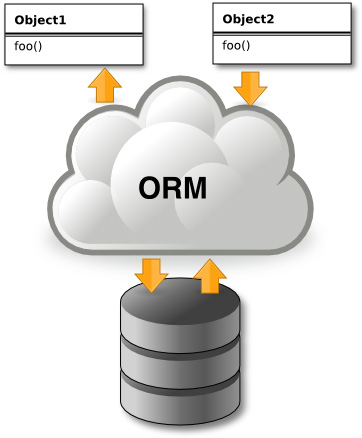
\includegraphics[width=12cm,height=12cm]{./IMAGENES/orm}
				\end{center}
Alberto Fernández.(2013).Aprende ya qué es un ORM:.[Figura].Recuperado de 
http://www.analyticaweb.com/desarrollo-web/aprende-ya-que-es-un-orm

			\end{figure}



\subsection{Características generales de los ORM. }
Entre las principales características se
encuentran las siguientes \citep {referencia05}:	
\begin{itemize}
\item Rapidez de desarrollo. ORM permite crear un modelo ajustado ya que lee
automáticamente el esquema de tablas y relaciones.
\item Abstracción del motor de base de datos. ayuda a que automáticamente las
consultas que se realicen en la base de datos se conviertan de registros a
objetos y viceversa y de esta forma adaptarse a los proveedores: (MYSQL,
ORACLE, POSTRESQL, ETC.). 
\item Lenguaje propio para consultas a la base de datos: las herramientas que
ofrece ORM para poder extraer los datos de la forma que se necesita (filtros,
ordenaciones, agrupaciones.
\item Proporciona una interfaz siendo más simples para el manejo de objetos a
través de su propio lenguaje de consulta [Anonimo]
\end{itemize}

\subsection{Patrón Repository}	
El patrón Repository  utiliza un repositorio para separar la lógica que recupera los datos y los mapea al modelo  de  entidades,  de  la  lógica  del    negocio  que  actúa  en  el  modelo.  El  repositorio  media  entre  la capa de fuente de datos y la capa de negocios de la aplicación; encuesta a la fuente de datos, mapea los datos obtenidos de la fuente de datos a la entidad de negocio y persisten los cambios de la entidad de negocio a la fuente de datos. 
Los repositorios son puentes entre los datos y las operaciones que se encuentran en distintos dominios. Un  repositorio  elabora  las  consultas  correctas  a  la  fuente  de  datos  y  mapea  los  resultados  a  las entidades de negocio expuestas externamente. Los repositorios eliminan las dependencias a tecnologías específicas proveyendo acceso a datos de cualquier tipo.
El patrón de diseño Repository puede ayudar a separar las capas de una aplicación web  ASP.NET ya que provee una arquitectura de 3 capas separadas,  lo que mejora el mantenimiento de la aplicación y ayuda a reducir errores.  Además facilita las pruebas unitarias.\citep {referencia02}	


\subsection{Patrón Active Record}
Active Record es un patrón en el cual, el objeto contiene los datos que representan a una fila (o tupla)
de nuestra tabla o vista, además de encapsular la lógica necesaria para acceder a la base de datos. De
esta forma el acceso a datos se presenta de manera uniforme a través de la aplicación (lógica de negocio
+ acceso a datos en una misma clase). En la figura 2 se muestra un esquema del patrón Active Record.
Una clase Active Record consiste en el conjunto de propiedades que representa las columnas de la tabla
más los típicos métodos de acceso como las operaciones CRUD (Create, Read, Update, Delete),
búsqueda (Find), validaciones, y métodos de negocio \citep {referencia06}.
Este patrón constituye la aproximación más obvia, poniendo el acceso a la base datos en el propio
objeto de negocio. De este modo es evidente como manipular la persistencia a través de él mismo. Gran
parte de este patrón viene de un Domain Model y esto significa que las clases están muy cercanas a la
representación en la base de datos. Cada Active Record es responsable de sí mismo, tanto en lo
relacionado con persistencia como en su lógica de negocio \citep {referencia02}.


\section{Ventajas y desventajas de utilizar ORM: }

\subsection{Ventajas:}
\begin{itemize}
\item Rapidez en el desarrollo. La mayoría de las herramientas actuales permiten la creación del modelo por
medio del esquema de la base de datos, leyendo el esquema, nos crea el modelo adecuado.Esto quita
mucho tiempo de “coding” repetitivo y que, seguro, el sistema hace mejor que nosotros, ya que los
humanos siempre cometemos fallos tontos. 
\item Abstracción de la base de datos. Al utilizar un sistema ORM, lo que conseguidos es separarnos
totalmente del sistema de Base de datos que utilicemos, y así si en un futuro debemos de cambiar de
motor de bases de datos, tendremos la seguridad de que este cambio no nos afectará a nuestro
sistema, siendo el cambio más sencillo. 
\item Reutilización. Nos permite utilizar los métodos de un objeto de datos desde distintas zonas de la
aplicación, incluso desde aplicaciones distintas. 
\item Seguridad. Los ORM suelen implementar sistemas para evitar tipos de ataques como pueden ser los
SQL injections
\item Mantenimiento del código. Nos facilita el mantenimiento del código debido a la correcta ordenación de
la capa de datos, haciendo que el mantenimiento del código sea mucho mas sencillo. 
\item Lenguaje propio para realizar las consultas. Estos sistemas de mapeo traen su propio lenguaje para
hacer las consultas, lo que hace que los usuarios dejen de utilizar la sentencias SQL para que pasen a
utilizar el lenguaje propio de cada herramienta. 
\end{itemize}

	\begin{figure}[H]
			\begin{center}
					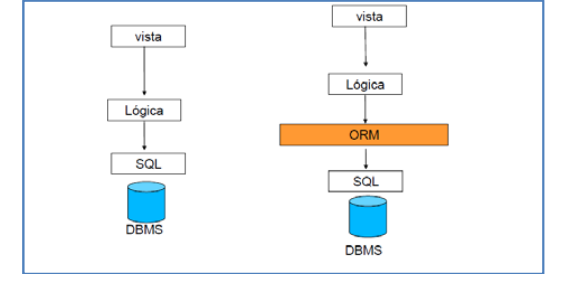
\includegraphics[width=12cm,height=10cm]{./IMAGENES/ventajas}
			\end{center}
			Alvial C,Saavedra Q,Valenzuela P(2011).ORM - Object Relational Mapping :.[Figura].Recuperado de 
			http://bit.ly/2lPY8i4
		\end{figure}
\subsection{Desventajas:}
\begin{itemize}
\item Rapidez en el desarrollo. La mayoría de las herramientas actuales permiten la creación del modelo por
medio del esquema de la base de datos, leyendo el esquema, nos crea el modelo adecuado.Esto quita mucho tiempo de “coding” repetitivo y que, seguro, el sistema hace mejor que nosotros, ya que los humanos siempre cometemos fallos tontos. 
\item Abstracción de la base de datos. Al utilizar un sistema ORM, lo que conseguidos es separarnos totalmente del sistema de Base de datos que utilicemos, y así si en un futuro debemos de cambiar de motor de bases de datos, tendremos la seguridad de que este cambio no nos afectará a nuestro
sistema, siendo el cambio más sencillo. 
\end{itemize}
\section{¿Que es NHIBERNATE?}
En pocas palabras, Nhibernate es un marco que nos permite hablar con una base de datos racional de una manera orientada a objetos. podemos almacenar (o como también solemos decir, "persistir") objetos en una base de datos y cargar esos objetos desde la base de datos más adelante. Nhibernate traduce nuestro lenguaje basado en objetos a un lenguaje que la base de datos entiende. es decir, nhibernate genera las declaraciones sql necesarias para insertar, actualizar, eliminar y cargar datos.
si usamos nhibernate, nunca tendremos que escribir ningún código que trate con hechos, aunque exista un desajuste de impedancia entre la forma en que desarrollamos aplicaciones en .NET y cómo funciona una base de datos. nhibernate ha abstraído este desajuste para nosotros. \citep {referencia07}

\section{Analisis}
{\bf {Easy installation}}
\\
 npm install sequelize\\
 npm install mysql

{\bf {Simple usage}}

\begin{figure}[H]
			\begin{center}
					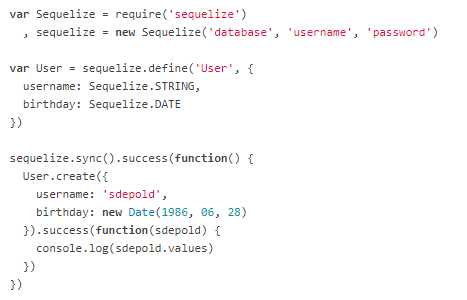
\includegraphics[width=14cm,height=10cm]{./IMAGENES/codigo}
			\end{center}
			SEQUELIZE(2019)Sequelize :.[Figura].Recuperado de 
			https://sequelize.readthedocs.io
		\end{figure}

\begin{figure}[H]
			\begin{center}
					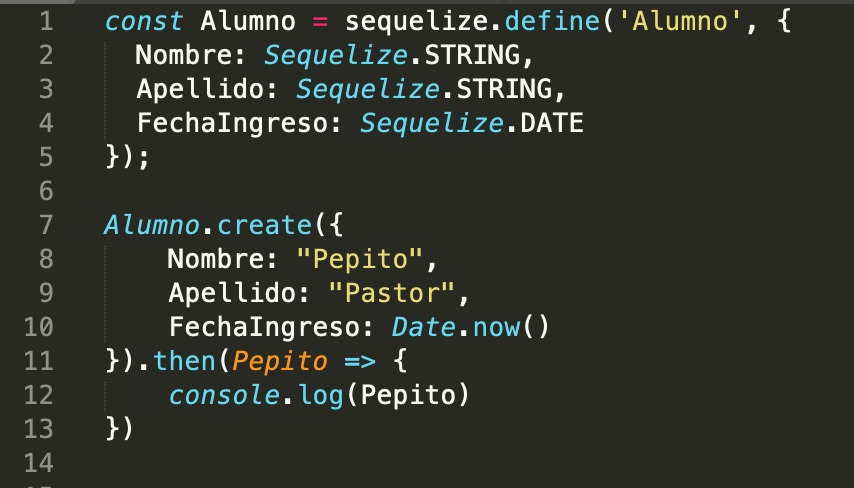
\includegraphics[width=14cm,height=10cm]{./IMAGENES/codigo2}
			\end{center}
			SEQUELIZE(2019)Sequelize :.[Figura].Recuperado de 
			https://sequelize.readthedocs.io
		\end{figure}

\begin{figure}[H]
			\begin{center}
					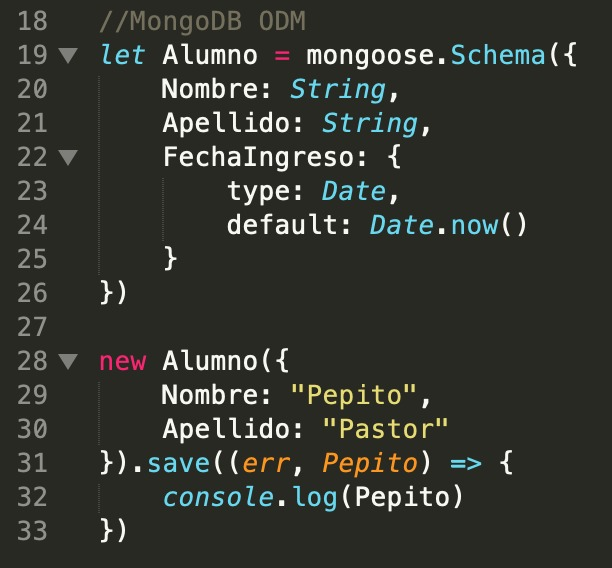
\includegraphics[width=14cm,height=10cm]{./IMAGENES/codigo3}
			\end{center}
			SEQUELIZE(2019)Sequelize :.[Figura].Recuperado de 
			https://sequelize.readthedocs.io
		\end{figure}


\section{Conclusion}
\begin{itemize}
\item Conclusion : \\

El uso de un ORM es una alternativa sumamente efectiva a la hora de trasladar el modelo conceptual
(orientado a objetos) al esquema relacional nativo de las bases de datos SQL. Evita la inclusión de
sentencias SQL embebidas en el código de la aplicación, lo que a su vez facilita la migración hacia otro
sistema gestor de bases de datos. 
\end{itemize}

	
	\newpage
	
	\bibliographystyle{apalike} 	
	\bibliography{BIBLIOGRAFIA}	 
\citep{referencia01}  
\citep{referencia02}  
\citep{referencia03}  
\citep{referencia04}  
\citep{referencia05}  
\citep{referencia06}  
\citep {referencia07}  
\end{document}

